\documentclass[t]{sdqbeamer}
%\documentclass[c]{sdqbeamer}

\usepackage{listings}
\usepackage{graphicx}
\usepackage{tabularx}
\usepackage{tikzsymbols}

\hypersetup{
	colorlinks=true,
	urlcolor=kit-green
}

% set sdqbeamer options
\titleimage{blender-render}
\groupname{} % rendered at the bottom center of each slide
\grouplogo{ae+satres}
\selectlanguage{english}

% define title etc.pp.
\title{Practical SAT Solving}
\subtitle{Lecture 1 \unimp{\normalfont --  Organization, Introduction, Incremental SAT Solving}}
\author{\underline{Ashlin Iser}, \underline{Dominik Schreiber}}
\date{April 20, 2026}

% define commands
\input{l00-commands.tex}


\begin{document}

\begin{frame}[title white horizontal, picture=logos/blender-render, kitlogo=rgb]
	\titlepage
\end{frame}

\begin{frame}{Organisation}
	\begin{itemize}\setlength{\itemsep}{1em}
		\item \textbf{14 lectures:} Mondays at 3:45 pm, room 301
		\item \textbf{7 exercises:} Tuesdays at 3:45 pm, room 301 (starting May 5, every other week)
		\item Bring your notebook if you can!
		\item Sign up: \url{https://campus.studium.kit.edu/ev/bZW-JQDwQ5qFbwb9yptSOQ}
		\item Find material (lecture plan, slides, exercises, code) on our course website:
		\begin{itemize}
			\item \large\url{https://satlecture.github.io/kit2026/}
		\end{itemize}
	\end{itemize}
\end{frame}

\begin{frame}{Organisers}
	\begin{itemize}\setlength{\itemsep}{1em}
		\item Lecturer: \textbf{Dr. Ashlin Iser} \hfill\unimp{\quad-- Post-doc at Algorithm Engineering group}\\
		Contact: \href{mailto:ashlin.iser@kit.edu}{ashlin.iser@kit.edu}\\[1ex]
		Expert in Boolean Reasoning and Empirical Algorithmics\\[1ex]
		Involved in this lecture since 2020 \unimp{(guest lectures before then)}\\[1ex]
		\item Lecturer: \textbf{Dr. Dominik Schreiber} \hfill\unimp{\quad-- Scalable Automated Reasoning (SatRes) group leader}\\
		Contact: \href{mailto:dominik.schreiber@kit.edu}{dominik.schreiber@kit.edu}\\[1ex]
		Expert in {parallel and distributed} SAT solving\\[1ex]
		Involved in this lecture since 2023 \unimp{(guest lectures before then)}\\[1ex]
		\item Co-manager of exercises: \textbf{Niccolò Rigi-Luperti} \hfill\unimp{\quad-- Doctoral researcher @ SAtRes group}\\
		Contact: \href{mailto:niccolo.rigi-luperti@kit.edu}{niccolo.rigi-luperti@kit.edu}\\[1ex]
		\item {Previous Lecturers}: {Prof. Carsten Sinz}, {Dr. Tom\'a\v{s} Balyo}\\
		\unimp{-- Founders of the Practical SAT Solving Lecture at KIT in 2015}
	\end{itemize}
\end{frame}

\begin{frame}{Homework, Competitions, and Oral Exam}
\begin{itemize}\setlength{\itemsep}{1em}
	\item You earn \highl{exercise points} for doing homework and coming to class with your solutions.
	\begin{itemize}
		\item For each exercise, the lucky ``referee'' is chosen randomly among all who stated that they prepared it
		\item No need to prepare a highly polished artifact! You need a \highl{clear idea and approach} (+ \highl{code} for practical exercises).
		\item Not being able to present an exercise after stating to be able \highl{invalidates all earned points so far}
	\end{itemize}
	\item You can earn \highl{at least 120 exercise points} during the semester (+ more bonus points).
	\begin{itemize}
		\item Some exercises may be in the form of small implementation contests.
		\item Bonus points are possible based on the type of exercise.
		\item We encourage group work! Jointly winning a contest gets each participant an equal share of the bonus points.
	\end{itemize}
	\item You must earn \highl{at least 60 points} to participate in the oral exam.
	\item Earning \highl{at least 120 points} will improve the grade of your \highl{passed oral exam} by one step.
\end{itemize}
\end{frame}

\begin{frame}{Goals of this Lecture}
Practical knowledge and transferable skills in the following areas:
\vspace*{5mm}
\begin{block}{Using SAT Solving}
	Solver usage, general encoding techniques, efficient CNF encodings of constraints, properties of encodings, \dots
\end{block}
\pause
\begin{block}{Practical Hardness of SAT}
Tractable classes, instance structure, hardest instances, proof complexity, \dots
\end{block}
\pause
\begin{block}{Methods for SAT Solving}
	Algorithms, and data structures, heuristics, implementation techniques, parallelization, proof formats, \dots
\end{block}
\pause
\begin{block}{Applications of SAT Solving}
	Hardware and software verification, planning and scheduling, security and cryptography, Explainable AI, \dots
\end{block}
\end{frame}

\begin{frame}{Plan for Today}
\begin{block}{Outline}
\begin{itemize}\setlength{\itemsep}{1em}
	\item Basic Definitions, History, and Complexity of SAT
	\item Applications of SAT Solving
	\item Examples from Mathematics and Computer Science
	\item Incremental SAT Solving
	\item Live Demo and Coding
\end{itemize}
\end{block}
\end{frame}


\begin{frame}{Basic Definitions}
In this lecture, propositional formulas are given in \emph{conjunctive normal form} (CNF), and if not, we convert them.\\[1em]
\begin{block}{CNF Formulas}
\begin{itemize}
	\item A \emph{CNF formula} is a conjunction (and = $\wedge$) of clauses.
	\item A \emph{clause} is a disjunction (or = $\vee$) of literals.
	\item A \emph{literal} is a Boolean variable $x$ (positive literal) or its negation $\overline{x}$ (negative literal).
\end{itemize}	
\end{block}
\begin{example}[CNF Formula]
\vspace{-3ex}
\begin{align*}
	F &= (\lnot x_1 \vee x_2) \wedge (\lnot x_1 \vee \lnot x_2 \vee x_3) \wedge (x_1)\\[1ex]
	\vars{F} &= \visible<2->{ \bigl\{ x_1, x_2, x_3 \bigr\} }\\[1ex]
	\lits{F} &= \visible<2->{ \bigl\{ x_1, \lnot x_1, x_2, \lnot x_2, x_3 \bigr\} }\\[1ex]
	\clss{F} &= \visible<2->{ \bigl\{ \{ \lnot x_1, x_2 \}, \{ \lnot x_1, \lnot x_2, x_3 \}, \{ x_1 \} \bigr\} }
\end{align*}
\end{example}
\end{frame}

\begin{frame}{Satisfiability}
The \emph{Satisfiability Problem} is to determine whether a given formula is satisfiable.\\[1ex]
A CNF formula $F$ is \emph{satisfiable} iff there exists a truth assignment to $\vars{F}$ that satisfies $F$.\\[1ex]
\begin{block}{Satisfying Assignment}
Given a CNF formula over variables $V$, a \emph{truth assignment} $\phi : V \longrightarrow \{ \top, \bot \}$ satisfies \dots \\[1em]
\dots~ a CNF formula if it satisfies all of its clauses \\[1ex]
\dots~ a clause if it satisfies at least one of its literals \\[1ex]
\dots~ a positive literal $x$ if $\phi(x)=\top$ (True)\\[1ex]
\dots~ a negative literal $\lnot x$ if $\phi(x)=\bot$ (False)\\[1ex]
\end{block}
\end{frame}

\begin{frame}{Satisfiability}
\begin{example}[Satisfiable or Unsatisfiable?]
	\vspace*{-3ex}
	\begin{align*}
		F_1 &= \{ \{ x_1 \} \}\\[1ex]
		F_2 &= \{ \{ x_1 \}, \{ \overline{x_1} \} \}\\[1ex]
		F_3 &= \{ \{ x_2, x_8, \overline{x_3} \} \}\\[1ex]
		F_4 &= \{ \{ x_1 \}, \{ \overline{x_2} \}, \{ x_2, \overline{x_1} \} \}\\[1ex]
		F_5 &= \{ \{ x_1, x_2 \}, \{ \overline{x_1}, x_2 \}, \{ x_1, \overline{x_2} \}, \{ \overline{x_1}, \overline{x_2} \} \}\\[1ex]
		F_6 &= \{ \{ \overline{x_1}, x_2 \}, \{ \overline{x_1}, \overline {x_2}, x_3 \}, \{ x_1 \} \}
	\end{align*}
\end{example}~\\
\pause
\highlow{Edge Cases:} What are the shortest satisfiable / unsatisfiable CNF formulas?
\end{frame}

\begin{frame}{Satisfiability}
\begin{columns}
\column{\kitthreecolumns}
	\begin{example}[Scheduling]
	Schedule a meeting of Adam, Bridget, Charles, and Darren considering the following constraints\\[1ex]
	\begin{itemize}\itemsep1ex
		\item Bridget cannot meet on Wednesday
		\item Adam can only meet on Monday or Wednesday
		\item Charles cannot meet on Friday
		\item Darren can only meet on Thursday or Friday
	\end{itemize}
	\end{example}
\column{\kitthreecolumns}	
	\begin{example}[CNF Encoding]
	\vspace{-2em}
	\begin{align*}
		\vars{F} = &\{ x_1, x_2, x_3, x_4, x_5 \}\\[1em]
		F = &\bigl\{ \visible<1->{ \{ \lnot x_3 \}, } \visible<2->{ \{ x_1, x_3 \}, } \visible<3->{ \{ \lnot x_5 \}, } \visible<4->{ \{ x_4, x_5 \}, }\\[3pt]
		% &\operatorname{AtMostOne}(x_1, x_2, x_3, x_4, x_5) \\[1ex]
		&\visible<5->{ ~\{ \lnot x_1, \lnot x_2 \}, \{ \lnot x_1, \lnot x_3 \}, \{ \lnot x_1, \lnot x_4 \}, \{ \lnot x_1, \lnot x_5 \},\\
		&~\{ \lnot x_2, \lnot x_3 \}, \{ \lnot x_2, \lnot x_4 \}, \{ \lnot x_2, \lnot x_5 \},\\
		&~\{ \lnot x_3, \lnot x_4 \}, \{ \lnot x_3, \lnot x_5 \},\\ 
		&~\{ \lnot x_4, \lnot x_5 \} } \bigr\}
	\end{align*}
	\end{example}~\\
	\only<6>{\highlow{Is this Scheduling Instance Satisfiable?}}
\end{columns}
\end{frame}

\begin{frame}{Complexity of Propositional Satisfiability}
\vspace*{-1em}
A decision problem is NP-complete if it is in NP and every problem in NP can be reduced to it in polynomial time.
\begin{block}{SAT is NP-complete (Cook-Levin Theorem)}
\begin{itemize}\itemsep1ex
	\item SAT is in NP\\
	\textbf{Proof:} solution can be checked in polynomial time
	\item Every problem in NP can be reduced to SAT in polynomial time\\
	\textbf{Proof:} encode the run of a non-deterministic Turing machine as a CNF formula
\end{itemize}
\end{block}~\\
\pause
\begin{block}{Consequences of NP-completeness of SAT}
\begin{itemize}\itemsep1ex
	\item We do not have a polynomial algorithm for SAT (yet) ~\cChangey{0}
	\item If $P \neq NP$ then we will never have a polynomial algorithm for SAT ~\cChangey{-1}
	\item All the known algorithms for SAT have exponential runtime in the \textbf{worst case} ~\cChangey{-2}
\end{itemize}
\end{block}~\\
\pause
\highlow{Try it yourself:} \url{http://www.cs.utexas.edu/~marijn/game/}
\end{frame}

\begin{frame}{History of Propositional Satisfiability}
\begin{block}{Historic Landmarks}
	\begin{itemize}\setlength{\itemsep}{1ex}
		\item \href{http://doi.acm.org/10.1145/321033.321034}{1960: DP Algorithm (first SAT solving algorithm)}
		% Davis, Putnam: A Computing Procedure for Quantification Theory
		\item \href{https://doi.acm.org/10.1145/368273.368557}{1962: DPLL Algorithm (improving upon DP algorithm)}
		% Davis, Logemann, Loveland: A Machine Program for Theorem-Proving
		\item \href{https://dl.acm.org/doi/10.1145/800157.805047}{1971: SAT is NP-Complete}
		% Cook: The Complexity of Theorem-Proving Procedures
		\item \href{http://www.aaai.org/Library/AAAI/1992/aaai92-068.php}{1992: Local Search Algorithm}
		Selman et al.: A New Method for Solving Hard Satisfiability Problems
		\item 1992: The First International SAT Competition (followed by 1993, 1996, since 2002 every year)
		\item 1996: The First International SAT Conference (Workshop) (followed by 1998, since 2000 every year)
		\item \href{https://doi.org/10.1109/12.769433}{1999: Conflict Driven Clause Learning (CDCL) Algorithm}
		% Marques-Silva, Sakallah: GRASP: A Search Algorithm for Propositional Satisfiability
	\end{itemize}
\end{block}
\begin{block}{Advancements}
	From 1992 to 2024, SAT solvers have improved by \highl{several orders of magnitude} in terms of feasible problem size.\\
	From 100 variables and 200 clauses to 21,000,000 variables and 96,000,000 clauses.
\end{block}
\end{frame}

\begin{frame}{SAT Conference}
	\begin{columns}
		\column{\kitfourcolumns}
		\centering
		\vspace*{-4mm}
		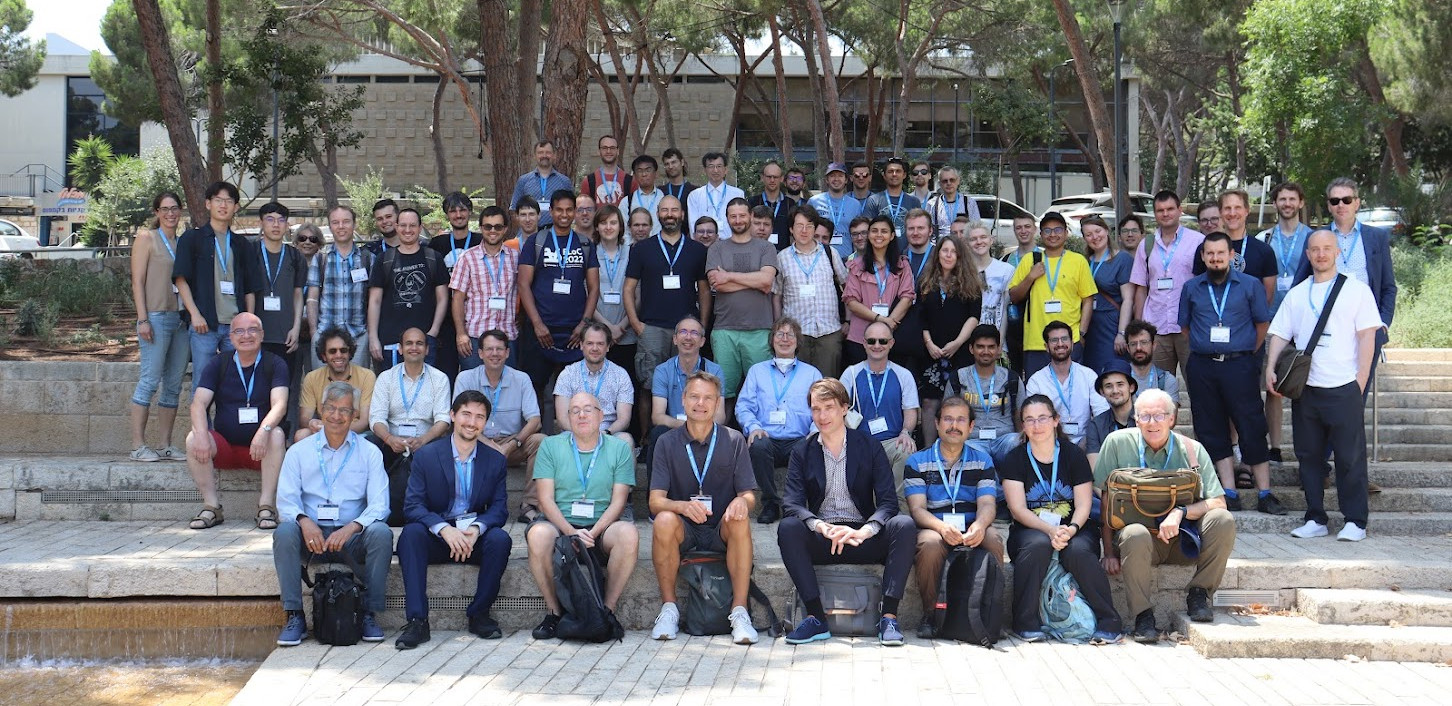
\includegraphics[width=18cm,trim=0 0.4cm 0 0.8cm,clip]{figures/l01/SAT2022-grouppicture-cropped.jpg}%
		\\[0.5cm]%
		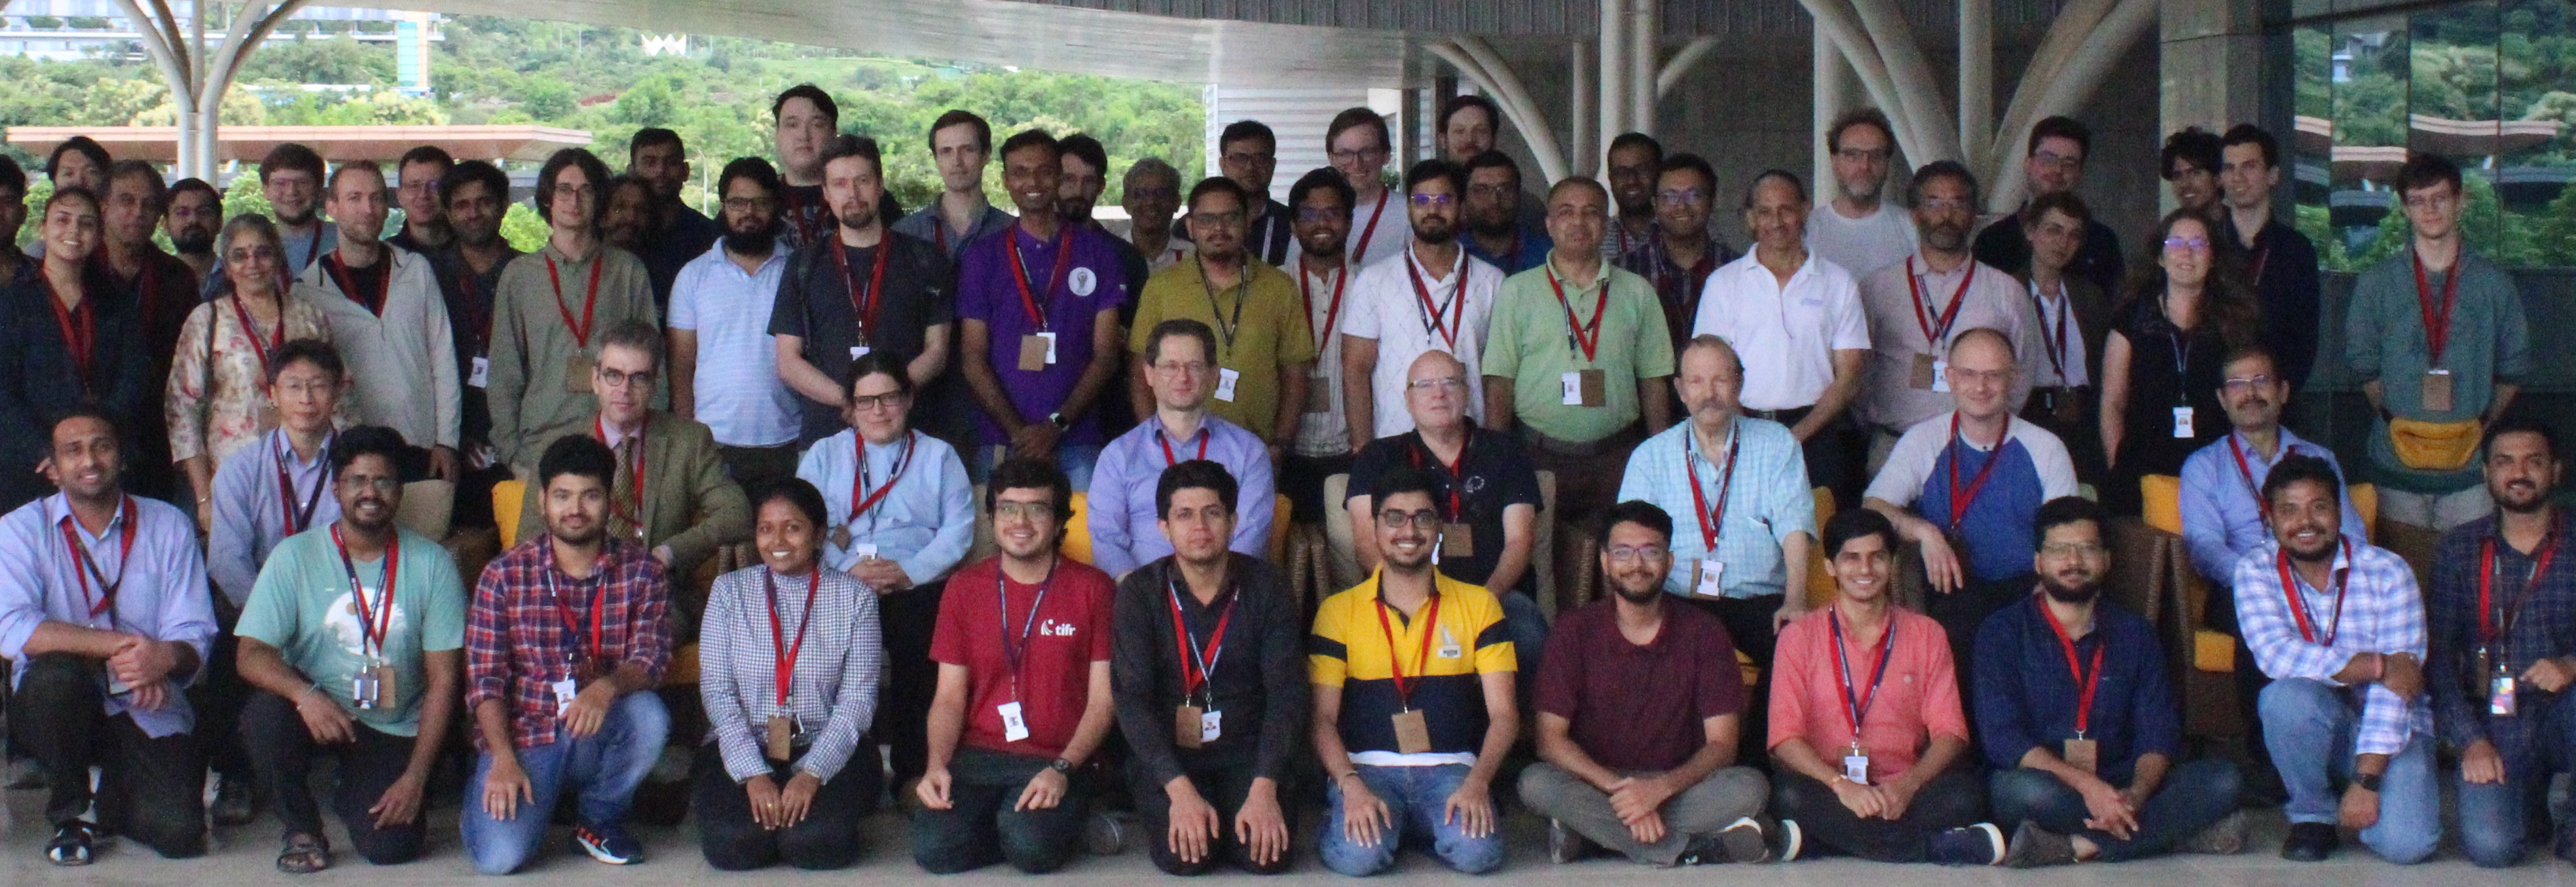
\includegraphics[width=16.5cm]{figures/l01/SAT2024pune.jpg}%
		\column{\kittwocolumns}
		2022, Haifa, Israel
		\\[4.8cm]
		2024, Pune, India
	\end{columns}
	\centering%
\end{frame}

\begin{frame}{Applications of SAT Solving}
\begin{minipage}{0.72\textwidth}
	\begin{itemize}\setlength{\itemsep}{1ex}
		\item Hardware verification and design
		\begin{itemize}
			\item Major hardware companies (Intel, \dots) use SAT to verify chip designs
			\item Computer Aided Design of electronic circuits
		\end{itemize}
		\item Software verification
		\begin{itemize}
			\item SAT-based SMT solvers are used to verify Microsoft software products\\
			and Amazon Web Services' core software libraries
			\item Embedded software in cars, airplanes, refrigerators,~\dots
			\item Unix utilities
		\end{itemize}
		\item Automated planning and scheduling
		\begin{itemize}
			%\item Good for small-to-medium sized, highly constrained problems
			\item Job shop scheduling, train scheduling, multi-agent path finding
		\end{itemize}
		\item Cryptanalysis
		\begin{itemize}
			\item Test/prove properties of cryptographic ciphers, hash functions
		\end{itemize}
		\item Number theoretic problems (Pythagorean triples, grid coloring)
		\item Solving other NP-hard problems (coloring, clique, \dots)
	\end{itemize}	
\end{minipage}%
\begin{minipage}{0.28\textwidth}
	
\includegraphics[width=\textwidth]{figures/l01/applications.png}
\end{minipage}
\end{frame}

\begin{frame}{SAT Solving in the News}
	\begin{minipage}{0.6\textwidth}
		\centering
		
\includegraphics[height=0.75\textheight]{figures/l01/triples-spiegel.png}
	\end{minipage}%
	\begin{minipage}{0.4\textwidth}
		\centering
		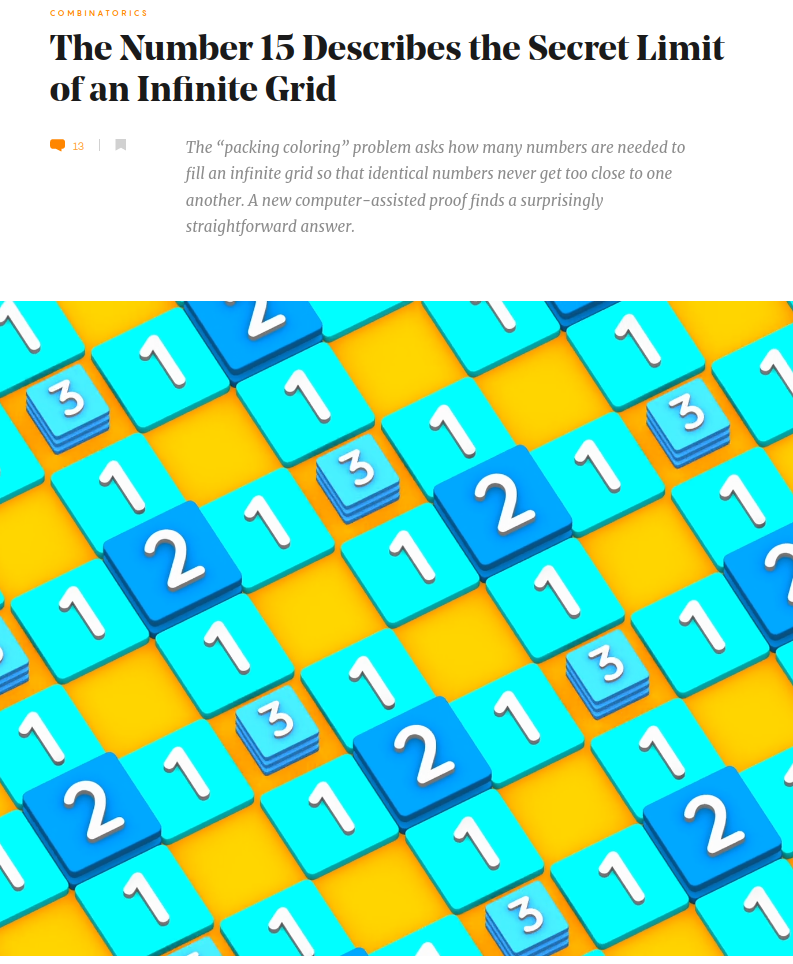
\includegraphics[height=0.75\textheight]{figures/l01/infinite-square-grid-article.png}
	\end{minipage}%
\end{frame}

\begin{frame}{Pythagorean Triples}
\begin{block}{Problem Definition}
Can we assign each integer $1,2,\ldots,n$\ \ to one of \highl{two colors} such that the following holds for all integers $a,b,c$:
\\
If \highl{$a^2+b^2=c^2$}, then $a,b$ and $c$ do not all have the same color.
\end{block}
\begin{itemize}
	\item Solution: \textbf{No!} Impossible for $n=7825$
	\item Proof obtained by a SAT solver has \highl{200 Terabytes} -- back then the largest Math proof yet
\end{itemize}
\pause
\vspace*{6mm}
\begin{block}{How to encode this?}
\pause
\begin{itemize}
	\item For each integer $i$, we have a Boolean variable $x_i$ which represents the color of $i$.
	\item For each $a,b,c$ such that $a^2+b^2=c^2$, encode two clauses: $(x_a \vee x_b \vee x_c)$
	and $(\overline{x_a} \vee \overline{x_b} \vee \overline{x_c})$
\end{itemize}
\end{block}
\end{frame}


\begin{frame}{Arithmetic Progressions}
\begin{block}{Problem Definition}
	Find a binary sequence $x_1, \dots, x_n$ that has no $k$ equally spaced zeroes and no $k$ equally spaced ones.
\end{block}
\pause
\begin{example}[$n=8, k=3$]
Find a binary sequence $x_1,\dots,x_8$ that has no three equally spaced zeroes and no three equally spaced ones.
\begin{itemize}
\item<2-> What about 01001011? \uncover<3->{No, the ones at $x_2, x_5, x_8$ are equally spaced.}
\item<4-> 6 Solutions: 00110011, 01011010, 01100110, 10011001, 10100101, 11001100.
\item<5-> Extending the problem to $n=9$ digits, \highl{no solution remains}. How can we show this with a SAT solver?
\item<6-> Encode what's forbidden: $x_2 x_5 x_8 \neq 111$ is the same as
   $(\overline{x_2} \lor \overline{x_5} \lor \overline{x_8})$.
\item<7-> Writing, e.g., $\bar 2 \bar 5 \bar 8$ for the clause $(\overline{x_2} \lor \overline{x_5} \lor \overline{x_8})$, we arrive
  at 32 clauses for the 9 digit sequence: \\
  $123, 234, \dots, 789, 135, 246, \dots, 579, 147, 258, 369, 159$,
  $\bar 1 \bar 2 \bar 3, \bar 2 \bar 3 \bar 4, \dots, \bar 7 \bar 8 \bar 9, \bar 1 \bar 3 \bar 5, \bar 2 \bar 4 \bar 6, 
  \dots, \bar 5 \bar 7 \bar 9, \bar 1 \bar 4 \bar 7, \bar 2 \bar 5 \bar 8, \bar 3 \bar 6 \bar 9, \bar 1 \bar 5 \bar 9$.
\end{itemize}
\end{example}
\end{frame}

\begin{frame}{Background: Van der Waerden Numbers}
Let's generalize our sequence to feature the numbers (``colors'') $\{0,1,\ldots,r-1\}$ \quad \unimp{(so far: $r=2$)}.
\begin{block}{Theorem (van der Waerden)}
For any $r, k \in \mathbb{N}^+$, there exists some $n \in \mathbb{N}^+$ such that:\\
Every sequence $x_1, \dots, x_n$ of numbers $0 \leq x_i < r$ has at least $k$ equally spaced positions with the same number.
\begin{itemize}
\item The smallest such $n$ is the \highl{van der Waerden number} $W(r,k)$.
\item For larger $r, k$, the numbers are only partially known.
\end{itemize}
\end{block}
\pause
\begin{example}[Van der Waerden Numbers]
\begin{itemize}
	\item We have seen that $W(2,3) = 9$.
	\item $W(2,6) = 1132$ was shown in \href{http://dx.doi.org/10.1080/10586458.2008.10129025}{[2008 by Kouril and Paul]} (using a SAT solver!)
	\item but $W(2,7)$ is yet unknown ($> 3\,703$).
	\item $2^{2^{r^{2^{2^{k+9}}}}}$ is an upper bound for $W(r,k)$ (shown in \href{http://dx.doi.org/10.1007/s00039-001-0332-9}{[2001 by Gowers]}).
\end{itemize}
\end{example}
\end{frame}

\begin{frame}{Graph Coloring}
\begin{example}[McGregor Graph, 110 nodes, planar]
	\textbf{Claim:} Needs $\geq$ 5 colors to color. \unimp{(Sc.\ American, \textbf{April} 1975, M.~Gardner's ``Mathematical Games'')}
	\begin{center}
		\includegraphics<1>[height=8.5cm]{figures/l01/macgregor-bw.jpg}
		%\includegraphics<2>[height=4.5cm]{figures/l01/macgregor_arb.jpg}
		\includegraphics<2>[height=8.5cm]{figures/l01/macgregor\_arb-colorblind-friendly.jpg}
	\end{center}
	\vspace*{1mm}
	\unimp{See: \url{https://www.cs.cmu.edu/~bryant/boolean/macgregor.html}}
\end{example}
\end{frame}

\begin{frame}{Graph Coloring: SAT Encoding}
\begin{block}{Definition: Graph Coloring Problem (GCP)}
Given an undirected graph $G=(V,E)$ and a number $k$, a \highl{$k$-coloring} assigns one of $k$ colors to each node\\
such that all adjacent nodes have a different color. The \highl{GCP} asks whether a $k$-coloring for $G$ exists.
\end{block}
\pause
\begin{block}{SAT Encoding}
\textbf{Variables:} 
\begin{itemize}
	\item<3-> use $k \cdot |V|$ Boolean variables $v_j$ for $v \in V, 1 \leq j \leq k$;\ \ $v_j$ is true iff node $v$ gets color $j$.
\end{itemize}
\textbf{Clauses:}
\begin{itemize}\setlength{\itemsep}{.5ex}
	\item<4-> Every node gets some color: 
	\item[]<5-> \quad $(v_1 \lor \cdots \lor v_k)\,$ for $v \in V$
	\item<6-> Adjacent nodes have different colors: 
	\item[]<7-> \quad $(\overline{u_j} \lor \overline{v_j})\,$ for ${u,v} \in E, 1 \leq j \leq k$
	\item<8-> Suppress multiple colors for a node: \highl{at-most-one constraints}
\end{itemize}
\end{block}
\end{frame}

\begin{frame}{Graph Coloring: Example}
\begin{example}[Graph Coloring Problem]
\begin{columns}
	\begin{column}{0.6\textwidth}
	\begin{itemize}
	\item $V = \{ u, v, w, x, y \}$
	\item Colors: red (=1), green (=2), blue (=3)
	\item Clauses: \\
	\textcolor{gray}{``every node gets a color''} \\
	$(u_1 \lor u_2 \lor u_3)$ \\
	$\quad\vdots$ \\ 
	$(y_1 \lor y_2 \lor y_3)$ \\ \vspace{0.5ex}
	\textcolor{gray}{``adjacent nodes have different colors''} \\
	$(\overline{u_1} \lor \overline{v_1}) \land \cdots \land (\overline{u_3} \lor \overline{v_3})$ \\
	$\quad\vdots$ \\
	$(\overline{x_1} \lor \overline{y_1}) \land \cdots \land (\overline{x_3} \lor \overline{y_3})$
	\end{itemize}
	\end{column}
	\begin{column}{0.4\textwidth}
	\begin{center}
		\includegraphics<1>[height=0.7\textwidth]{figures/l01/graph-coloring-1.pdf}
		\includegraphics<2>[height=0.7\textwidth]{figures/l01/graph-coloring-2.pdf}
	\end{center}
	\end{column}
\end{columns}
\end{example}
\end{frame}

\begin{frame}{Using a SAT Solver}
SAT solvers are command line applications that take as argument a text file with a formula.\\[1em]
\begin{example}[Input: DIMACS CNF format]
	\texttt{c comments, ignored by solver}\\
	\texttt{p cnf 7 22}\\
	\texttt{1 -2 7 0}\\
	\texttt{...}\\
	\texttt{-7 -3 -2 0}
\end{example}~\\
\pause
\begin{example}[Output]
	\texttt{c comments, usually some statistics about the solving}\\
	\texttt{s SATISFIABLE} \hspace{4em}\\
	\texttt{v 1 2 -3 -4}\\
	\texttt{v 5 -6 -7 0}\\
\end{example}
\end{frame}

\begin{frame}{Running a SAT Solver}
\highlow{Let's try it!}\\[1em]
\begin{enumerate}\setlength{\itemsep}{1em}
	\item Download and build a SAT solver:\\[1ex]
	\href{https://github.com/arminbiere/cadical}{CaDiCaL}, \href{https://github.com/arminbiere/kissat}{Kissat}, \href{https://github.com/niklasso/minisat}{Minisat}, \href{https://github.com/msoos/cryptominisat}{CryptoMinisat}, \href{https://maplesat.github.io/}{Maplesat}, \dots\\[1ex]
	In this lecture, we use: \href{https://github.com/arminbiere/cadical}{CaDiCaL}\\[1ex]
	\begin{itemize}\setlength{\itemsep}{1ex}
		\item Competitive performance
		\item Originally written by Armin Biere
		\item Highly educational, includes elaborate comments and references to the literature
		\item Reference implementations of the standard SAT solver interface: IPASIR
	\end{itemize}
	\item Download a SAT formula:\\[1ex]
	\href{https://benchmark-database.de}{Global Benchmark Database}
	\item Determine its satisfiability
\end{enumerate}
\end{frame}

\begin{frame}{Incremental SAT Solving}
There are many applications that require us to solve a sequence of similar SAT instances:\\[1ex] 
Software verification, planning, scheduling, MaxSAT, \dots\\[1em]
\begin{block}{Incremental SAT Solving}
\begin{itemize}\setlength{\itemsep}{0.5em}
	\item The SAT solver is initialized once with a formula
	\item Assumptions can be added before each call to \texttt{solve()}\\[1ex]
	$\rightarrow$ assumptions are literals that serve as a partial assignment to their variables
	\item Between \texttt{solve()} calls, new clauses can be added
	\pause
	\item Advantage 1: (De-)Initialization overheads removed
	\item Advantage 2: Keep preprocessed formula, learned clauses, dynamic heuristic parameters, \ldots
	\pause
	\item \highlo{Disadvantages}: \pause More complex solver logic, prevents some preprocessing / simplifications
\end{itemize}
\end{block}
\end{frame}

\begin{frame}{An Incremental SAT Solver Interface: IPASIR}
\vspace{-1em}
IPASIR = \textbf{R}e-entrant \textbf{I}ncremental \textbf{S}atisfiability \textbf{API} (acronym reversed)\\[1ex]
\begin{block}{IPASIR}
	\begin{itemize}\setlength{\itemsep}{0.5em}
		\item Defined for \href{https://doi.org/10.1016/j.artint.2016.08.007}{SAT Race 2015} to unify incremental SAT solver interfaces
		\item IPASIR has become a standard interface of incremental SAT solving
		\item Extension by User Propagators (UP): \href{https://doi.org/10.4230/LIPIcs.SAT.2023.8}{IPASIR UP}
		\item<2> Version 2 is in the works
	\end{itemize}
\end{block}~\\
\centering
\href{https://github.com/biotomas/ipasir}{
\includegraphics[width=.23\textwidth]{logos/ipasir.png}}
\qquad\qquad\qquad\qquad
\visible<2>{\href{https://github.com/ipasir2}{
\includegraphics[width=.23\textwidth]{logos/ipasir2.png}}}%
\end{frame}

\begin{frame}{IPASIR Functions}
	\def\arraystretch{1.5}
	\begin{tabularx}{\textwidth}{p{7em}X}
		\bf Function 	& \bf Description\\
		\hline
		\tt signature 	& return the name and version of the solver\\
		\tt init    	& initialize the solver, the pointer it returns is used for the rest of the functions\\
		\tt add 		& add clauses, one literal at a time\\
		\tt assume 		& add an assumption, the assumptions are cleared after a \texttt{solve()} call\\
		\tt solve 		& solve the formula, return SAT, UNSAT or INTERRUPTED\\
		\tt val 		& return the truth value of a variable (if SAT)\\
		\tt failed 		& returns true if the given assumption was part of reason for UNSAT\\
		\hline
	\end{tabularx}~\\[1em]
	For more details and examples of usage see \url{https://github.com/biotomas/ipasir}\\[1em]
	\visible<2>{\highlow{How to delete a clause?}}
\end{frame}

\begin{frame}{IPASIR Solver States}
\vspace{-1ex}
~~~~~~~~~~~~~~~~~~~~~~~~~~~~~~~~
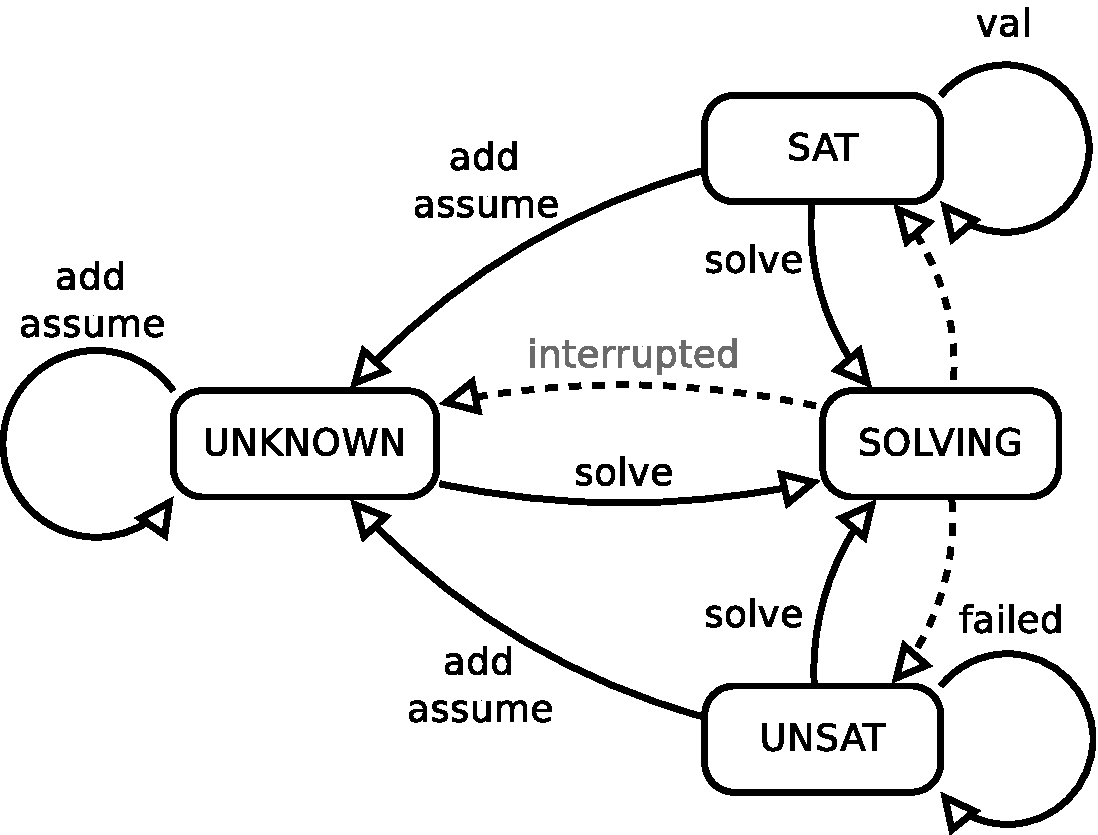
\includegraphics[height=.7\textheight]{figures/l01/ipasir.pdf}
\end{frame}

\begin{frame}{Essential Variables}
Given a CNF formula $F$ over variables $V := \vars{F}$, satifying assignments to $F$ can be partial, i.e.,\\
some variables in $V$ are not assigned but still the formula is satisfied.\\[1ex]
A variable $x$ is \emph{essential} if and only $x$ it has to be assigned (True or False) in each satisfying assignment.\\[1em]

\begin{example}[Enumerating Essential Variables]
\begin{itemize}\setlength{\itemsep}{1em}
	\item Create the \emph{Dual Rail Encoding} of $F$:\\[1ex]
	\begin{itemize}\setlength{\itemsep}{1ex}
		\item For each variable $x$, add two new variables $x_P$ and $x_N$
		\item Replace each positive (negative) occurrence of $x$ with $x_P$ ($x_N$)
		\item Add a clause $(\overline{x_P} \vee \overline{x_N})$ (meaning $x$ cannot be both true and false)
	\end{itemize}
	\item For each variable $x$, solve the formula with the assumptions $\overline{x_P}$ and $\overline{x_N}$.\\[1ex]
	If the formula is UNSAT under these assumptions then $x$ is essential.
\end{itemize}
\end{example}%
%~\\\highlow{Let's implement it!}\\[1em]
\end{frame}

\end{document}
